\documentclass[letterpaper,12pt]{article}
\usepackage[top = 1in, bottom = 1in, left = 0.5in, right = 1in]{geometry}
\usepackage{inputenc}
\usepackage{graphicx}
\usepackage{amsmath}
\usepackage{amsfonts}
\usepackage{caption}
\usepackage{color}
\usepackage{listings}
\usepackage[framed,numbered,autolinebreaks,useliterate]{mcode}
%opening
\author{Gowtham Garimella}

\makeatletter
\newcommand\ackname{Acknowledgements}
\if@titlepage
  \newenvironment{acknowledgements}{%
      \titlepage
      \null\vfil
      \@beginparpenalty\@lowpenalty
      \begin{center}%
        \bfseries \ackname
        \@endparpenalty\@M
      \end{center}}%
     {\par\vfil\null\endtitlepage}
\else
  \newenvironment{acknowledgements}{%
      \if@twocolumn
        \section*{\abstractname}%
      \else
        \small
        \begin{center}%
          {\bfseries \ackname\vspace{-.5em}\vspace{\z@}}%
        \end{center}%
        \quotation
      \fi}
      {\if@twocolumn\else\endquotation\fi}
\fi
\makeatother

\newcommand{\executeiffilenewer}[3]{%
\ifnum\pdfstrcmp{\pdffilemoddate{#1}}%
{\pdffilemoddate{#2}}>0%
{\immediate\write18{#3}}\fi%
}
\newcommand{\includesvg}[1]{%
\executeiffilenewer{#1.svg}{#1.pdf}%
{inkscape -z -D --file=#1.svg %
--export-pdf=#1.pdf --export-latex}%
\input{#1.pdf_tex}%
}

\title{EN.530.603 Applied Optimal Control \\HW \#3 Solutions}
\graphicspath{{./figures/}}
\begin{document}
\maketitle

\begin{enumerate}

  %%%%%%%%%%%%%%%Question 1%%%%%%%%%%%%%%%%%%%%%%%%
  \item Given system dynamics:
  \begin{align*}
   \dot x_1(t) &= x_2(t)\\
   \dot x_2(t) &= -a x_2(t) + u(t) \\
   a > 0 \quad |u(t)| &\le 1 \quad x(t_f) = 0\\
  \end{align*}
  To minimize:
  \begin{align*}
   J = \int_{t_0}^{t_f} \gamma + |u(t)| dt \quad \gamma > 0\\
  \end{align*}
  \begin{enumerate}
   \item The Hamiltonian and adjoint equations are as follows:
   \begin{align*}
    H &= \gamma + |u| + \lambda_1 ( x_2) + \lambda_2 (-a x_2 + u)\\
    \dot \lambda &= -\nabla H_x\\
    \Rightarrow \begin{bmatrix}
                 \dot \lambda_1\\
                 \dot \lambda_2\\
                \end{bmatrix} &= 
                \begin{bmatrix}
                 0 \\
                 -\lambda_1 + a \lambda_2\\
                \end{bmatrix}\\
    \nabla H_u &= \pm 1 + \lambda_2 \quad \text{(Does not provide u)}\\
    H^*_u &= |u| + \lambda_2 u \quad \text{(Choose u to minimize this)}\\
    \Rightarrow u &= \begin{cases}
                      1 & \mbox{if}\enskip \lambda_2 > 1\\
                      0 & \mbox{if}\enskip 1 > \lambda_2 > -1\\
                      -1 & \mbox{if}\enskip -1 > \lambda_2 \\
                     \end{cases}
   \end{align*}
   \item From the dynamics of the lagrange multipliers:
   \begin{align*}
    \lambda_1 &= c_1\\
    \lambda_2 &= c_2 e^{at} + \frac{c_1}{a}\\
   \end{align*}
   From the Boundary conditions, since the final time is free,
   \begin{align*}
    H(t_f) &= 0 \quad \Rightarrow \gamma + |u_f| + \lambda_{2f} u_f = 0\\
    \Rightarrow \lambda_2(t_f) &= \begin{cases}
                                  -(1+\gamma) &\mbox{if } u_f = 1 \\
                                  (1+\gamma) & \mbox{if } u_f = -1\\
                                 \end{cases}
   \end{align*}
   $u_f$ cannot be equal to zero in the above equation. Given that $\lambda_2(t)$ is exponential,
and the final value is either greater than 1 or less than -1, there can be atmost \textbf{two
switches}. So the optimal control sequences are: \{-1,0,1\} \{0,1\} \{1\} \{1,0,-1\} \{0,-1\} \{-1\}
 
   \item The singular points where the control becomes undefined is given when $\lambda_2 =
\{-1,0,1\}$. Given the form of $\lambda_2$ as:
   \begin{equation*}
    \lambda_2 = c_2 e^{at} + \frac{c_1}{a}\\
   \end{equation*}
  $\lambda_2$ is continuously increasing or decreasing unless $c_2 = 0$ in which case the boundary
conditions ensure that:
  \begin{equation*}
   \lambda_2 = \lambda_2(t_f) = \pm (1 + \gamma)
  \end{equation*}
  which is not any of the singular values. Thus the value of $\lambda_2$ cannot stay at the singular
values for any time interval. Thus there are no \textbf{singular intervals}.
  
  \item To determine the optimal control law we look at the switching curves:
   \begin{enumerate}
    \item u = -1 always. Then 
    \begin{align*}
     \dot x_2(t) &= -a x_2 - 1 \quad x_{2f} = 0\\
     x_2(t) &= (1/a) [e^{-a(t-t_f)} - 1]\\
     \dot x_1(t) &= x_2 \quad x_{1f} = 0\\
     x_1(t) &= (1/a) [(1/a)e^{-a(t-t_f)} - (t-t_f))]\\
     \Rightarrow x_1(t) &= \frac{1}{a^2} [-ax_2 + log(ax_2 + 1)] \quad x_2 > (-1/a)\\
    \end{align*}
    \item u = -1 always. Then similar to above,
    \begin{align*}
      x_1(t) = \frac{-1}{a^2} [ax_2 + log(1 - ax_2)] \quad x_2 < (1/a)\\
    \end{align*}
    \item u = 0. Then
    \begin{align*}
     \dot x_2 &= -a x_2 \quad \dot x_1 = x_2 \\
     \Rightarrow x_1 &= -(x_2 - x_{20})/a  + x_{10}
    \end{align*}
    This is just a straight line with slope (-1/a).
   \end{enumerate}
  \end{enumerate}
   These combine to provide the switching curves shown in Fig[\ref{fig1}]. The general family of curves for u = 1,-1, 0 are
plotted in Fig[\ref{fig2}]. Based on the control strategy u(t) and given that the  optimal control sequences noted in part (c)
the optimal control law is devised based on the example scenarios present in Figures[\ref{fig3}][\ref{fig4}]
    \begin{align*}
     u = \begin{cases}
          \{-1,0,1 \} \mbox{ or } \{0,1 \} & \mbox{if } x_10 < \frac{1}{a^2} [-ax_20 + log(1 + ax_20)] \enskip\&\enskip x_20 > 0\\
          \{-1,0,1 \}  & \mbox{if } x_10 < \frac{-1}{a^2} [ax_20 + log(1 - ax_20)]\enskip\&\enskip x_20 \le 0\\
          \{1,0,-1 \} \mbox{ or } \{0,-1 \} & \mbox{if } x_10 > \frac{-1}{a^2} [ax_20 + log(1 - ax_20)] \enskip\&\enskip x_20 <
0\\
          \{1,0,-1 \}  & \mbox{if } x_10 > \frac{1}{a^2} [-ax_20 + log(1 + ax_20)] \enskip\&\enskip x_20 > 0\\
         \end{cases}\\
    \end{align*}
    The times for which the sequence of controls are to be executed can be found by forward integrating the dynamics and ensuring
that $x(t_f) = 0$.

    \begin{figure}[h!]
      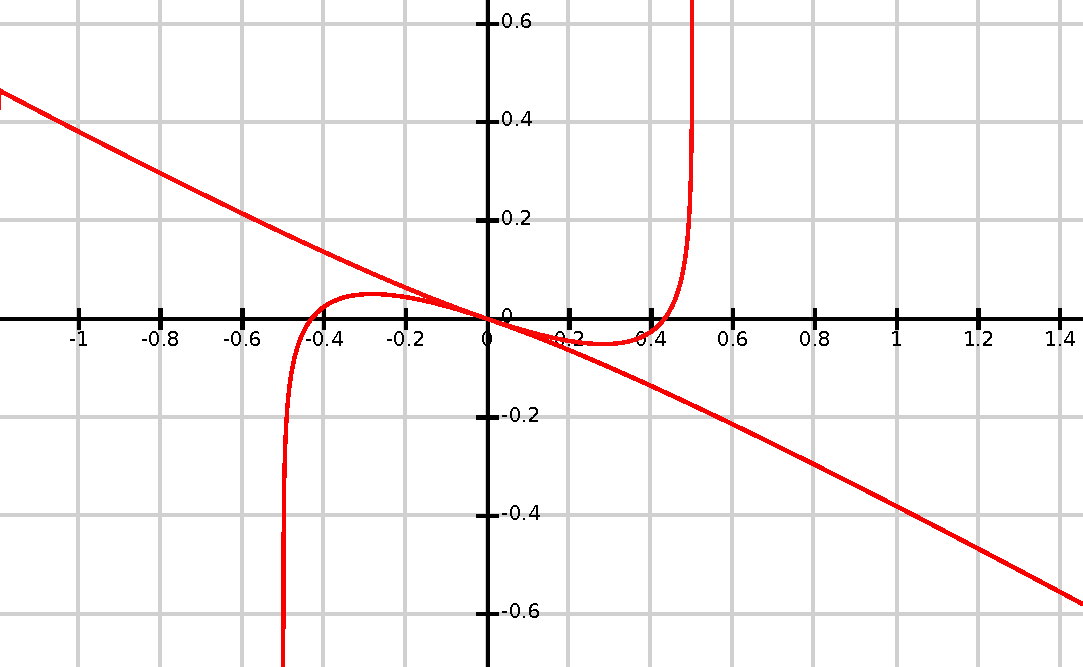
\includegraphics[width=\linewidth]{pic2.pdf}
      \caption{The switching curves $x_1(t)$ vs $x_2(t)$ passing through origin}
      \label{fig1} 
    \end{figure}
      \begin{figure}[h!]
      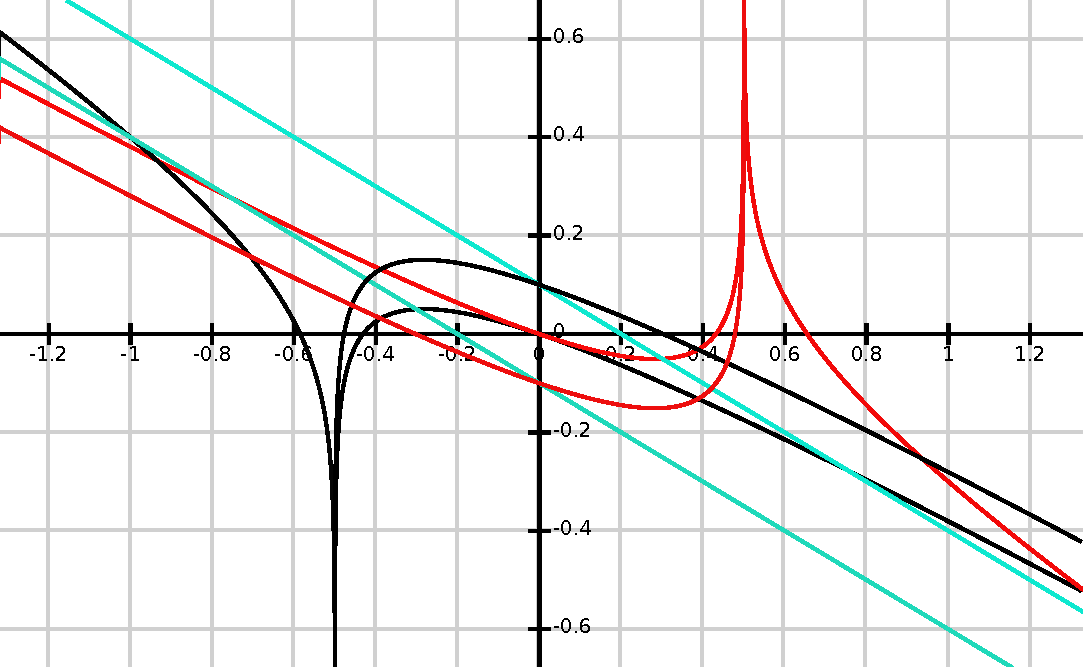
\includegraphics[width=\textwidth, height = 10cm, keepaspectratio= true]{pic1.pdf}
      \captionsetup{singlelinecheck=off}
      \caption{Plot of combined Family of curves (a) Red Lines show the family of u = -1 curves (b) Green Lines show the family of
u = 0 curves (b) Black Lines show the family of u = 1 curves }
      \label{fig2} 
    \end{figure}
     \begin{figure}[h!]
      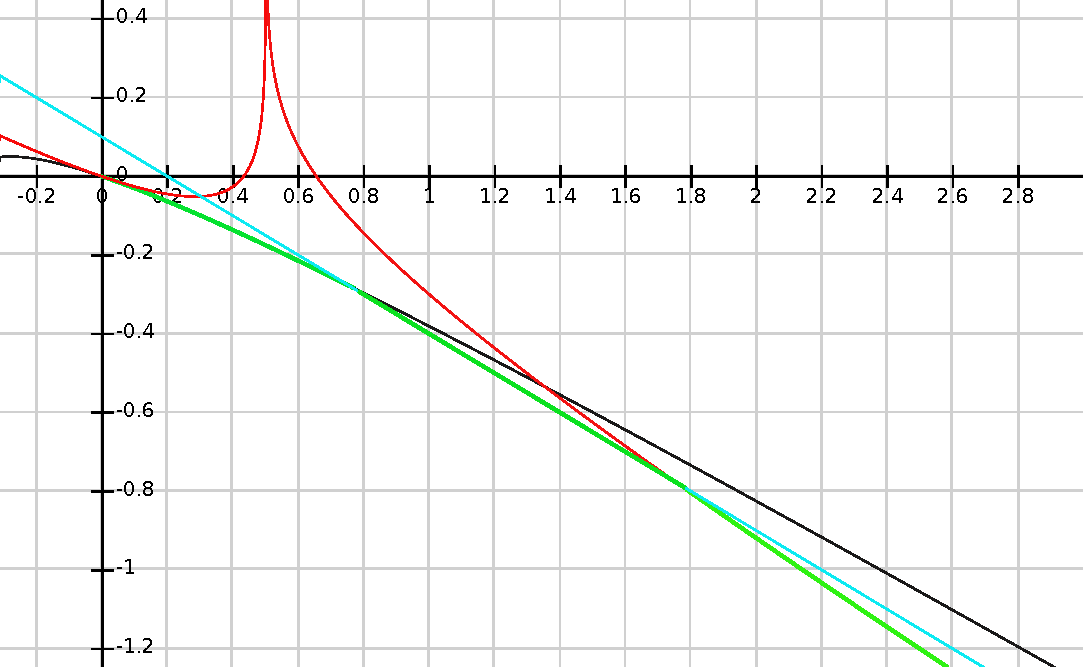
\includegraphics[width=\linewidth, height = 10cm,  keepaspectratio= tru]{pic3.pdf}
      \caption{Example Scenario 1 optimal control sequence(-1,0,1)}
      \label{fig3} 
    \end{figure}
    \begin{figure}[h!]
      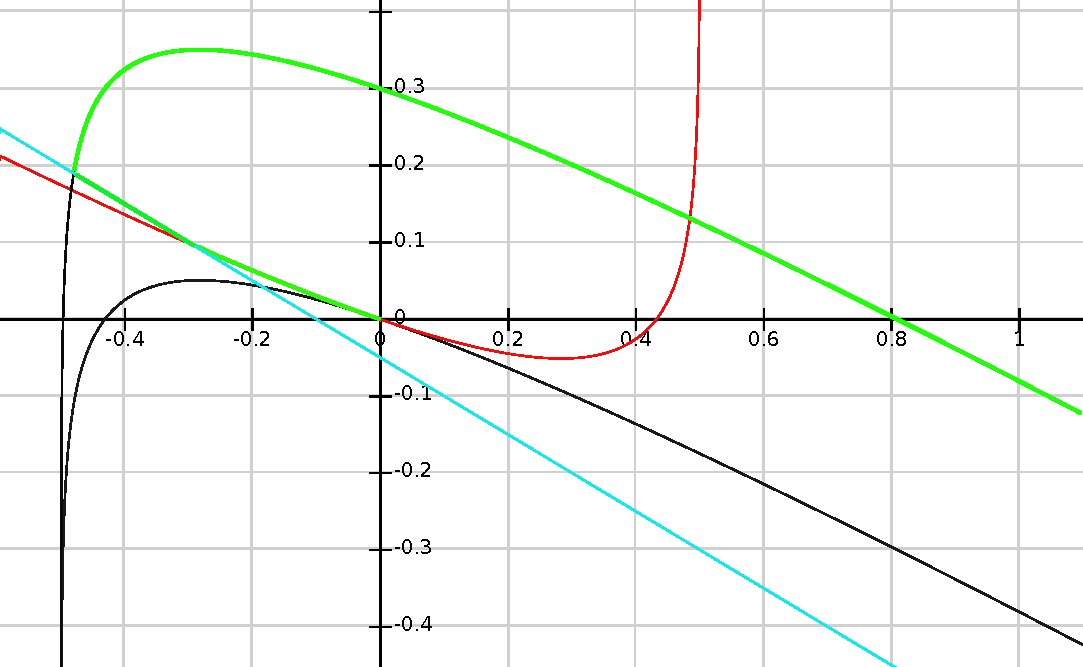
\includegraphics[width=\linewidth, height = 10cm,  keepaspectratio= tru]{pic4.pdf}
      \caption{Example Scenario 2 optimal control sequence(1,0,-1)}
      \label{fig4} 
    \end{figure}
    \newpage
  %%%%%%%%%%%%%%%Question 2%%%%%%%%%%%%%%%%%%%%%%%%
    \item Given to minimize:
      \begin{align*}
       J = \lVert x(t_f)\rVert^2 
      \end{align*}
      subjected to the dynamics of the system:
	\begin{align*}
	\dot x = Ax + Bu, \quad x(0) = x_0, \quad t_f \mbox{ given}
	\end{align*}
    Equating related parts of the problem to the general optimization setting, we have:
      \begin{align*}
       \Phi = x(t_f)^T x(t_f) \quad H = \lambda^T (Ax+Bu) 
      \end{align*}
      The necessary optimality conditions required are :
      \begin{align*}
       \dot \lambda &= - \nabla H_x = - A^T \lambda \\
       \partial H_u &= \lambda^T B\\
       \lambda(t_f) &= \nabla_x \Phi(t_f) = 2 x(t_f)
      \end{align*}
      Since the optimal control cannot be obtained by $\partial H_u$ we use poincare conditions to find the control on the
boundaries:
     \begin{align*}
      u^* &= min H^* (u) = \lambda^T B u\\
      \Rightarrow u^* &= \begin{cases}
                         -1 & \lambda^T B > 0\\
                         1 & \lambda^T B < 0\\
                         \mbox{singular} & \lambda^T B = 0
                        \end{cases}\\
     \end{align*}
     This shows that the control for optimization is bang bang i.e the control either stays at +1 or -1 if $\lambda^T B \neq0$.
     
     For the double integrator the dynamics of the system are given as follows:
       \begin{align*}
        A = \begin{bmatrix}
             0 & 1 \\
             0 & 0 \\
            \end{bmatrix} \quad 
        B = \begin{bmatrix}
             0 \\
             1
            \end{bmatrix}\\
       \end{align*}
       The control is then given as :
	 \begin{equation*}
	\Rightarrow u^* = \begin{cases}
                         -1 & \lambda_2 > 0\\
                         1 & \lambda_2 < 0\\
                         \mbox{singular} & \lambda_2 = 0
                        \end{cases}\\  
	 \end{equation*}
    Now to find the general trajectories for this case, we look at the system and multiplier dynamics. 
    \begin{align*}
    \dot \lambda_1 &= 0\\
    \dot \lambda_2  &= - \lambda_1\\
    \lambda(t_f) &= 2 x(t_f) \\
    \Rightarrow \lambda_1 &= \mbox{ const } \\
    \Rightarrow \lambda_2 &= -\lambda_1 t + c_1 \\
    \end{align*}
    The linearity of $\lambda_2$ implies that we can atmost switch twice. But when $\lambda_2$ goes to zero we cannot decide on
the control since it is singular. Thus the possible optimal control sequences are $\{1\}, \{-1\}, \{1, -1\}, \{-1,1\},\{0\}$.  

If the control is always +1 then initial position should lie on:
  \begin{align*}
   x_1(t0) &= x_2(t0)^2 \quad x_2(t0) < 0 \\
   \mbox{OR } x_1(t0) &< 0 , \enskip x_2(t0) < 0 \quad \mbox{ (Third Quadrant with small } t_f)
  \end{align*}
else if the control is always -1 then initial position should lie on:
  \begin{align*}
   x_1(t0) &= -x_2(t0)^2 \quad x_2(t0) > 0\\
   \mbox{OR } x_1(t0) &> 0 , \enskip x_2(t0) > 0 \quad \mbox{ (First Quadrant with small } t_f)
  \end{align*}
else the control sequence is \{-1,1\} then the initial position should lie in:
  \begin{align*}
   x_1(t0) &> x_2(t0)^2 \enskip x_2(t0) < 0\\
   \mbox{OR } x_1(t0) &> 0 , \enskip x_2(t0) > 0 \quad \mbox{ (First Quadrant with large } t_f)
  \end{align*}
else the control sequence is \{-1,1\} then the initial position should lie in:
  \begin{align*}
   x_1(t0) &< -x_2(t0)^2 \enskip x_2(t0) > 0\\
   \mbox{OR } x_1(t0) &< 0 , \enskip x_2(t0) < 0 \quad \mbox{ (Third Quadrant with large } t_f)
  \end{align*}


One important fact that makes this optimal control problem a lot simpler is that, when the time $t_f$ given is long enough to reach origin
using any of the above sequences then we do not have to execute any more control since we already have reached the goal i.e least possible distance to origin. This fact
shows that there is minimum final time for every position beyond which the control sequence do not change. 

The switching curves which go to zero are shown in Fig[\ref{fig5}] and the optimal trajectories for some of the sequences
discussed above are shown in Fig[\ref{fig6}]
  \begin{figure}[h!]
    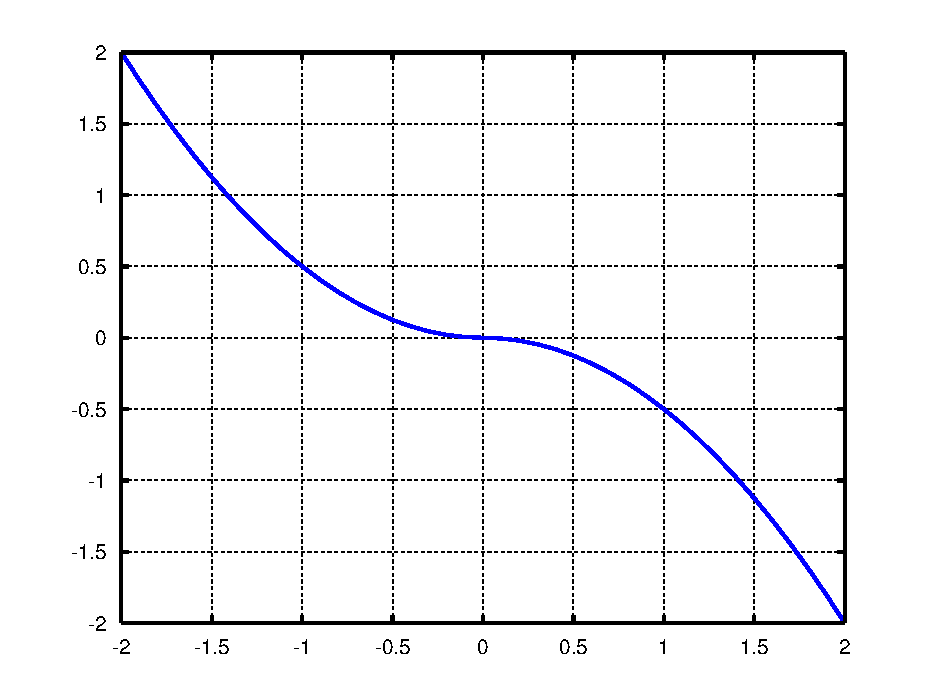
\includegraphics[width=\linewidth]{pic5.pdf}
    \caption{The switching curves $x_1(t)$ vs $x_2(t)$ passing through origin}
    \label{fig5} 
  \end{figure}
  \begin{figure}[h!]
    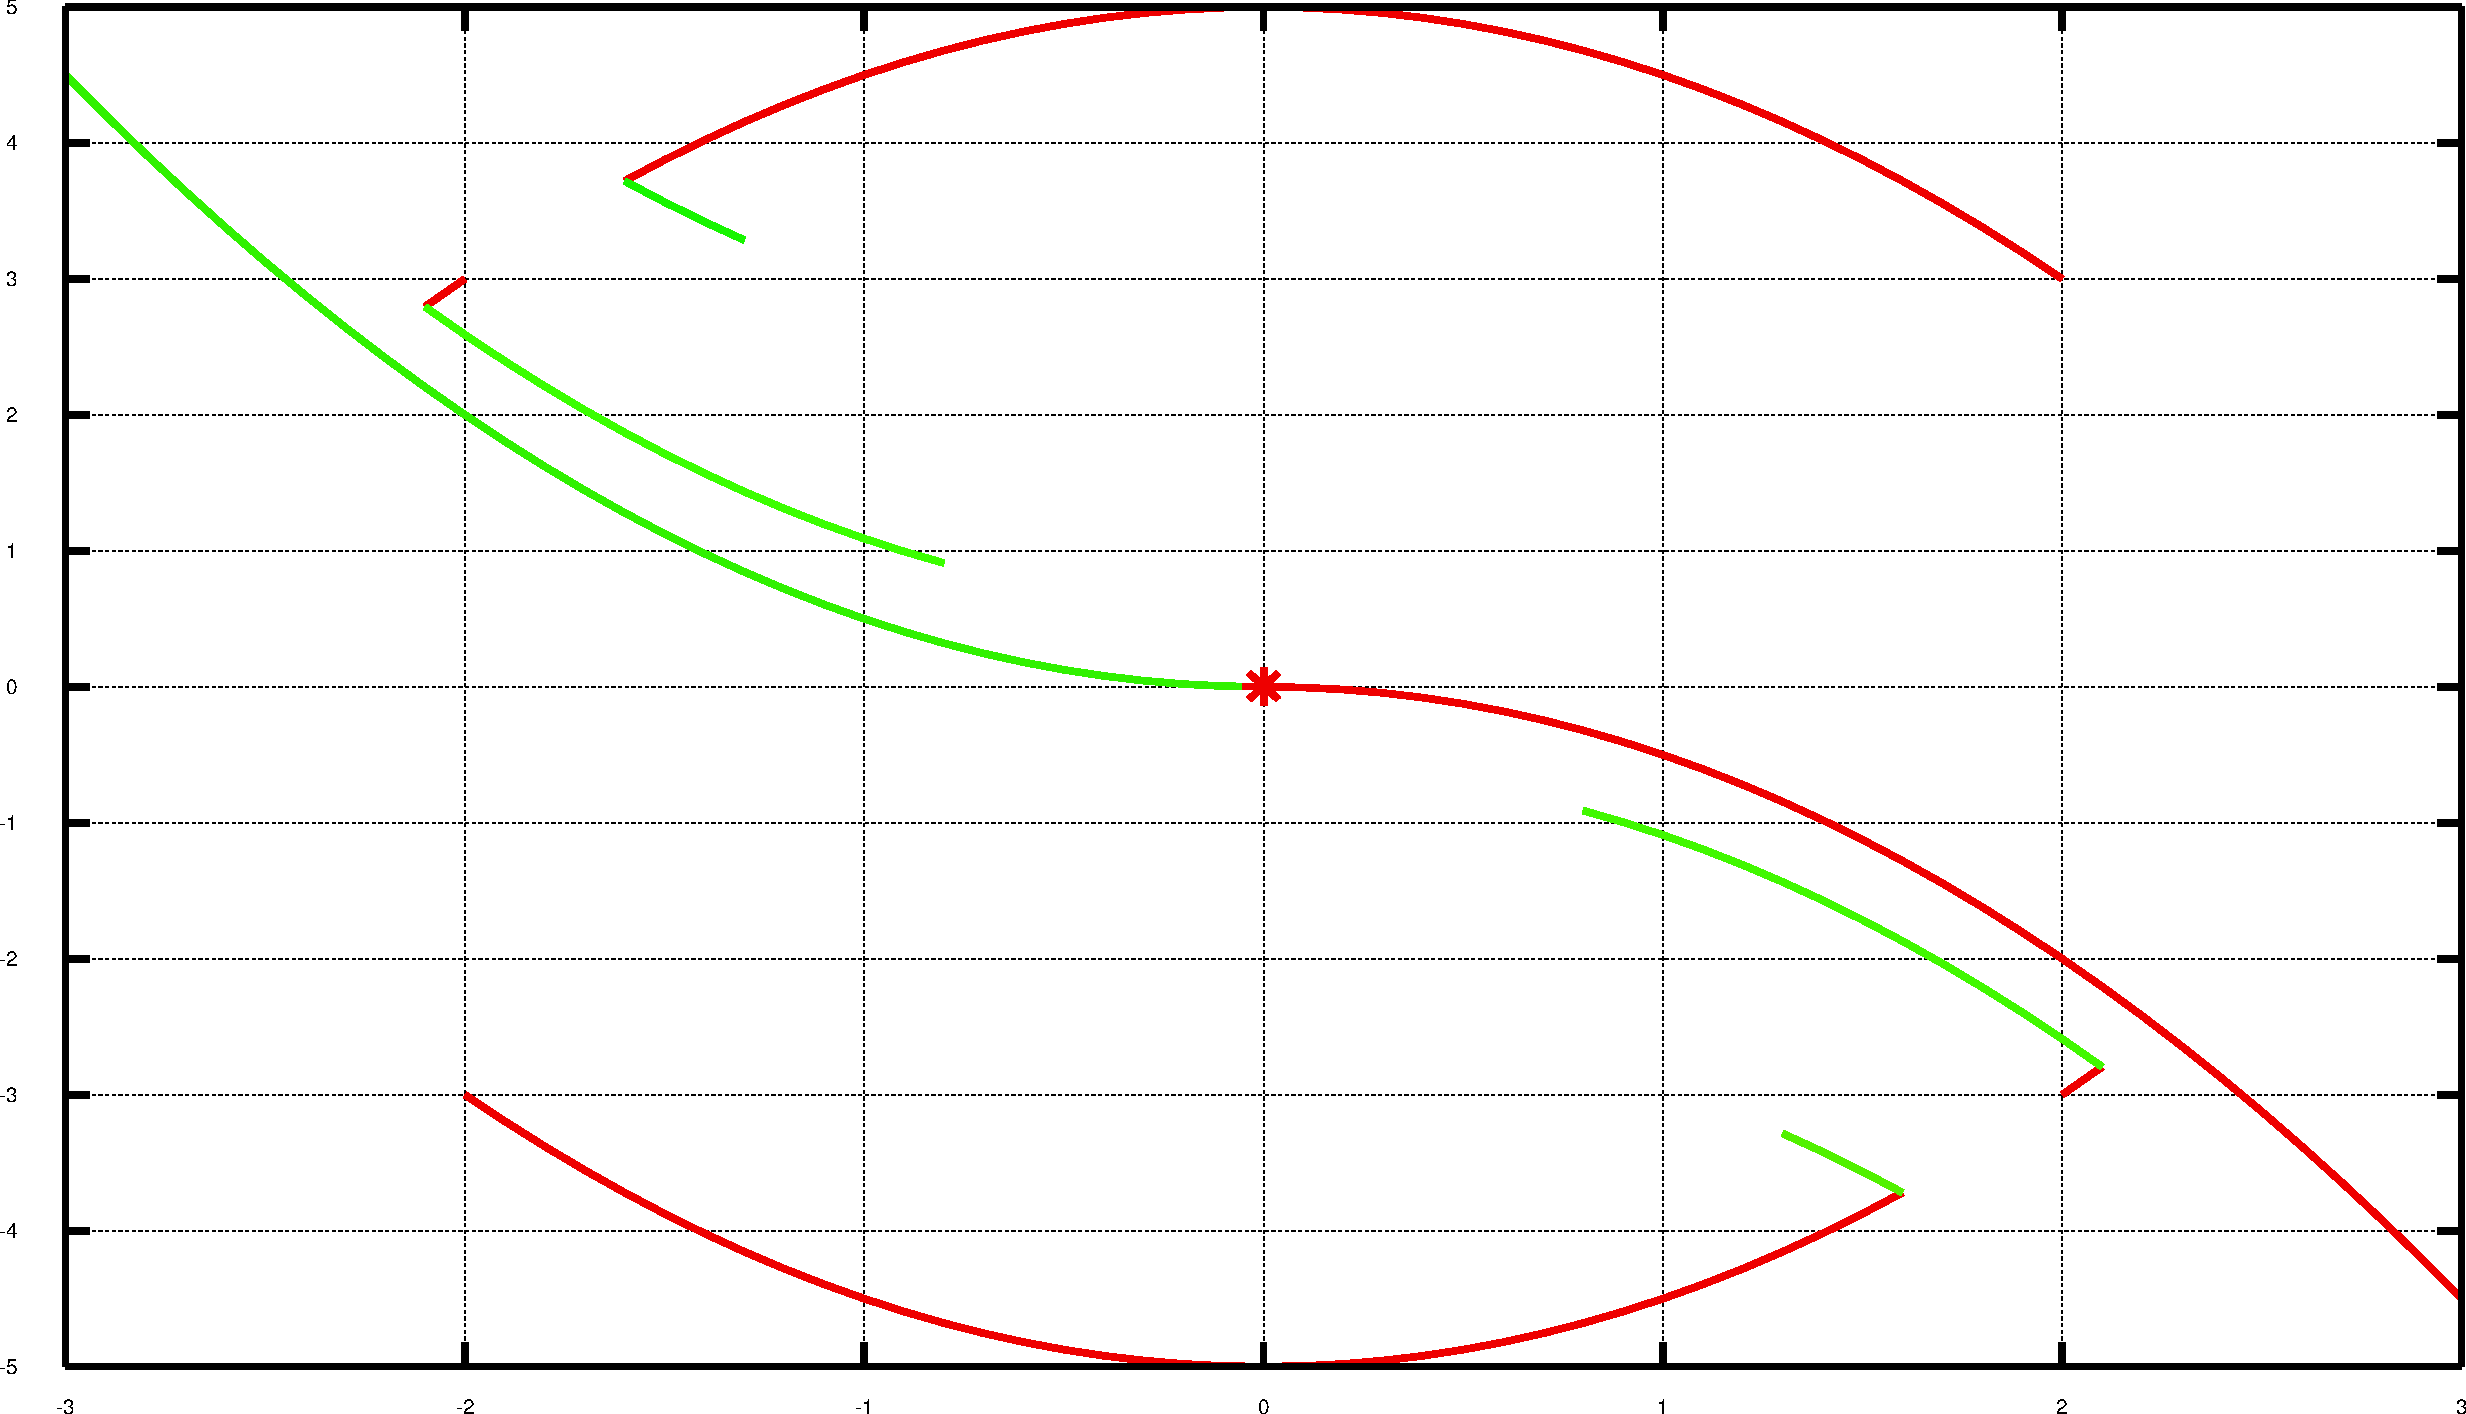
\includegraphics[width=\linewidth]{pic6.pdf}
    \caption{The optimal trajectories  $x_1(t)$ vs $x_2(t)$ depicting various control sequences plotted by simulating the
dynamics in MATLAB.(a) The red curves represent u = -1 and green represent u = +1 (b) Once the paths reach origin, they do not
move any further even if the final time is increased. The control remains zeros thereafter.}
    \label{fig6} 
  \end{figure}
%decide on the figures when u get time 

  %%%%%%%%%%%%%%%Question 3%%%%%%%%%%%%%%%%%%%%%%%%
\item Given a robotic arm with two degrees of freedom ($\theta_1, \theta_2$). The state of the arm is given as:
  \begin{equation*}
   x = (\theta_1, \theta_2, \dot \theta_1, \dot \theta_2)
  \end{equation*}
  The forward kinematics of the RR manipulator is given as:
    \begin{equation*}
     p_t = \begin{pmatrix}
            cos(\theta_1) l_1 + cos(\theta_1 + \theta_2) l_2 \\
            sin(\theta_1) l_1 + sin(\theta_1 + \theta_2) l_2 \\
           \end{pmatrix}
    \end{equation*}
   The state inequality for obstacle avoidance is given as:
     \begin{align*}
      \lVert p_t - p_0 \rVert^2 &\ge r^2 \\
      c(x(t),t) = r^2 - (p_t - p_0)^T (p_t - p_0) &\le 0 \\
     \end{align*}
    Since the above state inequality does not directly say anything about the control, we differentiate c(x(t),t) until controls
show up. Thus the new inequality are obtained as:
  

  \begin{align*}
  \dot c &= 2{(p_0-p_t)}^T \dot p_t  = 2{(p_0-p_t)}^T (\partial_x{p_t} \dot x) \\
  \mbox{Where } \partial_x p_t &= \begin{pmatrix}
                                  -sin(\theta_1)l_1 - sin(\theta_1 + \theta_2) l_2 & - sin(\theta_1 + \theta_2) l_2 & 0 & 0\\
                                  cos(\theta_1)l_1 + cos(\theta_1 + \theta_2) l_2 & cos(\theta_1 + \theta_2) l_2 & 0 & 0\\
                                 \end{pmatrix}\\
  \Rightarrow  \dot c &= 2(p_0 - p_t)^T \begin{pmatrix}
                                  -sin(\theta_1)l_1 \dot \theta_1 - sin(\theta_1 + \theta_2) l_2 (\dot \theta_1 + \dot \theta_2)\\
                                  cos(\theta_1)l_1 \dot \theta_1 + cos(\theta_1 + \theta_2) l_2 (\dot \theta_1 + \dot \theta_2)\\
                                       \end{pmatrix}\\
  \end{align*}
  Since $\dot c$  does not have information about u1 and u2 we differentiate again to get 
  \begin{align*}
   \ddot c &= 2(p_0 - p_t)^T(\partial_x(\partial_x p_t \dot x) \dot x) + 2 (\partial_x p_t \dot x)^T (\partial_x p_t \dot x)\\ 
  \partial_x(\partial_x p_t) &= \begin{pmatrix}
				    -l_1 cos(\theta_1) \dot \theta_1 - l_2 cos(\theta_1 + \theta_2)(\dot \theta_1 +
\dot \theta_2)& \cdots \\
 \hfill -l_2 cos(\theta_1 + \theta_2)  (\dot \theta_1 + \dot \theta_2) & -l_1 sin(\theta_1) -l_2sin(\theta_1 +
\theta_2) & -l_2sin(\theta_1+ \theta_2)\\[6pt]
                                  -l_1 sin(\theta_1) \dot \theta_1 - l_2 sin(\theta_1 + \theta_2)(\dot \theta_1 + \dot \theta_2)
& \cdots\\ 
\hfill -l_2 sin(\theta_1 + \theta_2)  (\dot \theta_1 + \dot \theta_2) &  l_1 cos(\theta_1) +  l_2cos(\theta_1 + \theta_2)
& l_2cos(\theta_1 + \theta_2)\\[6pt]
                                 \end{pmatrix}\\
   \partial_x(\partial_x p_t)\dot x &= \begin{pmatrix}
					-l_1 c_1 \dot \theta_1^2 -l_2 c_{12} (\dot \theta_1 + \dot \theta_2)^2 + u_1 (-l_1 s_1 -
l_2 s_{12}) + u_2 (-l_2 s_{12})\\
					-l_1 s_1 \dot \theta_1^2 -l_2 s_{12} (\dot \theta_1 + \dot \theta_2)^2 + u_1 (l_1 c_1 +
l_2 c_{12}) + u_2 (l_2 c_{12})\\
                                      \end{pmatrix}\\
   \partial_x p_t \dot x &= \begin{pmatrix}
                                  -sin(\theta_1)l_1 \dot \theta_1 - sin(\theta_1 + \theta_2) l_2 (\dot \theta_1 + \dot \theta_2)\\
                                  cos(\theta_1)l_1 \dot \theta_1 + cos(\theta_1 + \theta_2) l_2 (\dot \theta_1 + \dot \theta_2)\\
                                       \end{pmatrix}\\
  \end{align*}
 The above inequality has $u_1$ and $u_2$. Hence the collection $(c \enskip\dot c\enskip \ddot c) \le 0$ gives the state
control inequality conditions which must be satisfied on the boundary. Thus the constraints are:
  \begin{align*}
      c(x(t),t) &= r^2 - (p_t - p_0)^T (p_t - p_0) \le 0 \\
   \dot c(x(t),t) &= 2(p_0 - p_t)^T \begin{pmatrix}
                                  -sin(\theta_1)l_1 \dot \theta_1 - sin(\theta_1 + \theta_2) l_2 (\dot \theta_1 + \dot \theta_2)\\
                                  cos(\theta_1)l_1 \dot \theta_1 + cos(\theta_1 + \theta_2) l_2 (\dot \theta_1 + \dot \theta_2)\\
                                       \end{pmatrix} \le 0\\
    (p_0 - p_t)^T &\begin{bmatrix}
 -l_1 sin(\theta_1) -l_2sin(\theta_1 + \theta_2) & -l_2sin(\theta_1+ \theta_2)\\
  l_1 cos(\theta_1) +  l_2cos(\theta_1 + \theta_2) & l_2cos(\theta_1 + \theta_2)\\
                  \end{bmatrix} 
                  \begin{bmatrix}
                   u_1 \\
                   u_2 \\
                  \end{bmatrix} \le - (\partial_x p_t \dot x)^T (\partial_x p_t \dot x) - (p_0 - p_t)^T M(x)
  \end{align*}
\item Given rocket dynamics as :
\begin{align*}
 \dot x_1(t) &= \frac{cu(t)}{x_2(t)} - \frac{D}{x_2(t)} \\
 \dot x_2(t) &= - u(t) \\
\end{align*}
 To maximize the range of rocket, the optimization problem is set as:
 \begin{align*}
   \mbox{maximize }J = \int_{t_0}^{t_f} x_1(t) dt \quad x(t_0) \mbox{ and } x(t_f) \mbox{ are given}
 \end{align*}
 and terminal time is free. Equating to the general optimal control setting we get:
 \begin{align*}
  H = x_1(t) + \lambda_1( \frac{cu(t)}{x_2(t)} - \frac{D}{x_2(t)} ) + \lambda_2 ( - u(t)) \\
 \end{align*}
 Since terminal time is free and there are no terminal constraints, $H(t_f) = 0$ and since H is not explicitly dependent on time (t), H = const = 0 throught the interval.
 The adjoint equations for the control problem are given as:
 \begin{align*}
  \dot \lambda_1 &= - 1 \\
  \dot \lambda_2 &= -\lambda_1\left(\frac{cu - D}{{x_2}^2}\right)
 \end{align*}
 To investigate the possibility of singular control intervals, we try to find the necessary optimal conditions:
 \begin{align*}
  H_u = \frac{c \lambda_1}{x_2} - \lambda_2\\
 \end{align*}
 Since $H_u$ does not provide the optimal control directly, we check if we are on the boundaries.
 \begin{align*}
  \mbox{maximize }H^*(u) = \left(\frac{c \lambda_1}{x_2} - \lambda_2\right) u \\
 \end{align*}
 Since the only boundary condition on u is $u(t) \ge 0$ , we are on the boundary of the control only when $\frac{c \lambda_1}{x_2} - \lambda_2 < 0$ and will be singular when it is an equality. So when we are not on the boundary, we are at a singular interval since we cannot decide the control based on either directly solving for $H_u$ or using the minimum principle. The optimal control in such a case is decided by differentiating $H_u$ until control explicitly appears and set it to zero. The number of times we differentiate is called order of singularity. For the current case:
 \begin{align*}
  \dot H_u &= \frac{-c \lambda_1}{{x_2}^2} (-u) + \frac{c(-1)}{x_2} - (-\lambda_1)\left(\frac{cu - D}{{x_2}^2}\right)\\
  \Rightarrow \dot H_u &= \frac{-c}{x_2} + \frac{\lambda_1 D}{{x_2}^2}\\
  \Rightarrow \ddot H_u &= \frac{c}{{x_2}^2} (-u) - \frac{2\lambda_1 D}{{x_2}^3}(-u) - \frac{D}{{x_2}^2}
 \end{align*}
 For singular intervals described above, optimal control is given by setting $\ddot H_u = 0$:
 \begin{align*}
  u^* = \frac{D x_2}{2 \lambda_1 D - c x_2  }
 \end{align*}






\end{enumerate} 
\vfill
\begin{acknowledgements}
I hereby declare that I have not discussed this homework with anyone. The solutions written here are
my own work and  from lecture notes and sample code provided by the professor. Any 
external references are mentioned in the text.
\flushright Gowtham Garimella
\end{acknowledgements}




\end{document}
